
% Document class and font size
%-----------------------------------------------
\documentclass[10pt, oneside]{article}

% Aesthetics and colors
%-----------------------------------------------
\usepackage[hmargin = 1.25cm, vmargin = 1.5cm]{geometry} 
\usepackage[utf8]{inputenc}  % for the portuguese characters 
\usepackage[none]{hyphenat} % no hyphenated words
\usepackage[usenames,dvipsnames]{xcolor} 
\usepackage{microtype} % to optimize spacing
\usepackage{array}
\usepackage{lmodern}
\usepackage{tikz} % For photo placement
\usepackage{fancyhdr}
\pagestyle{fancy}
\fancyhf{}
\newcommand\tab[1][1cm]{\hspace*{#1}}
\usepackage{multirow}
\usepackage{longtable}

% Fonts and tweaks for XeLaTeX
%-----------------------------------------------
\usepackage{fontspec,xltxtra}
\usepackage{xltxtra}
\usepackage{xunicode}
\defaultfontfeatures{Mapping=tex-text}
%\setsansfont[Scale=MatchLowercase,Mapping=tex-text]{Gill Sans} % Font my name at the top


%%% Couleurs
\definecolor{baseline-gray}{HTML}{f0f2f2}
\definecolor{baseline-black}{HTML}{212222}
\definecolor{baseline-blue}{HTML}{2d3bff}
\definecolor{baseline-red}{HTML}{ff5043}

% url color and font
%-----------------------------------------------
\usepackage[colorlinks,urlcolor=baseline-black,bookmarks=false,hypertexnames=true]{hyperref}
\urlstyle{same} 

% Customized section headers
%-----------------------------------------------
\usepackage{titlesec} % Allows creating custom \section's
	\titleformat{\section}{\bf\color{baseline-black}
	\scshape\Large\raggedright}{}{0em}{}[\color{black}\titlerule]
	\titlespacing{\section}{0pt}{0pt}{5pt} % Spacing around titles
\renewcommand{\headrulewidth}{0pt} % Get rid of the default rule in the header

%contact info
\newcommand{\cvemail}{david.beauchemin.5@ulaval.ca}
\newcommand{\cvphonenumber}{(514) 250-3616}
\newcommand{\cvlinkedin}{https://www.linkedin.com/in/david-beauchemin-918343108/}
\newcommand{\github}{https://github.com/davebulaval}

% Customized subsection headers
%-----------------------------------------------
\titleformat{\subsection}{\bfseries\large\raggedright}{}{0em}{}[\color{black}]
\titlespacing{\subsection}{0pt}{2.5pt}{2.5pt}

% Settings for the vertical timeline
%-----------------------------------------------
\newcolumntype{L}{>{\raggedleft}p{0.14\textwidth}}
\newcolumntype{R}{p{0.8\textwidth}}
\newcommand\VRule{\color{baseline-gray}\vrule width 0.5pt}

\usepackage{fontawesome}

%---------------------------------------------------------
% ----- Begginning of the documment ---------------
%---------------------------------------------------------
\begin{document}

% Name in the top center
%-----------------------------------------------
\par{\centering{\bf\sffamily\Huge David Beauchemin}\\\vspace{2pt}


% Colored boxes with personal info
%----------------------------------------------- 

\par{\centering
	\href{mailto:\cvemail}{\faEnvelopeO} \,\, \href{mailto:\cvemail}{\cvemail}\\
	\faPhone \,\, \cvphonenumber \\
	\href{\github}{\faGithub}\,\, \href{\github}{Voir GitHub} \\
	\href{\cvlinkedin}{\faLinkedinSquare}\,\, \href{\cvlinkedin}{Voir profil}\\
}

\vspace{10pt}

% Formal education
%-----------------------------------------------
\section*{Études}

\begin{tabular}{L!{\VRule}R}
  2020 -- \tab[.7cm] & \textbf{Doctorat en informatique | Apprentissage automatique | Traitement automatique du langage naturel}\\
  \multirow{1}{*}{
\includegraphics[scale=0.1]{images/UL_P.pdf} \tab[0.6cm]} &  Université Laval \\
                                & \href{https://graal.ift.ulaval.ca/}{GRAAL - Groupe de Recherche en Apprentissage Automatique de l'Université Laval}\\
                                &\\[-6pt]
                    
	2018 -- 2020           & \textbf{Maîtrise en informatique | Apprentissage automatique | Traitement automatique du langage naturel}\\
	\multirow{1}{*}{
\includegraphics[scale=0.1]{images/UL_P.pdf} \tab[0.6cm]}  &  Université Laval \\
								  & \href{https://graal.ift.ulaval.ca/}{GRAAL - Groupe de Recherche en Apprentissage Automatique de l'Université Laval}\\
								  & Sujet mémoire: \textit{Détection de doublons parmis des informations non structurées provenant de sources de données externes}\\
								  &\\[-6pt]
	                      
	2015 -- 2018           & \textbf{Baccalauréat en actuariat} \\
	\multirow{1}{*}{
\includegraphics[scale=0.1]{images/UL_P.pdf} \tab[0.6cm]}  &  Université Laval \\[-6pt]
\end{tabular}

\vspace{10pt}

% Experience
%-----------------------------------------------
\section*{Expériences}

\subsection{Profesionnelle}
\begin{tabular}{L!{\VRule}R}
2020 -- \tab[.7cm]   &{\bf {Chercheur en IA appliquée en traitement automatique du langage naturel}}\\
	\multirow{1}{*}{
\includegraphics[scale=0.075]{images/Baseline.png} \tab[1.1cm]}					& Coopérative Baseline en intelligence artificielle\\
	& Recherche appliquée de solution en IA pour des clients \& formation sur mesure en IA\\
	&\\[-6pt]
2019 -- \tab[.7cm]   &{\bf {Développeur}}\\
\multirow{1}{*}{
\includegraphics[scale=0.15]{images/poutyne.png} \tab[0.18cm]}& \href{https://poutyne.org/}{Poutyne}\\
& Développement de fonctionnalité \\ 
&\\[-6pt]

2019 -- \tab[.7cm]   &{\bf {Fondateur, recherchiste et intervieweur}}\\
	\multirow{1}{*}{
\includegraphics[scale=0.025]{images/OpenLayer.png} \tab[0.8cm]}& \href{https://www.youtube.com/channel/UCB3tYpZ1ojiqAroyDN05Cyw}{OpenLayer podcas}t\\
	& Création de contenu en IA \\ 
	&\\[-6pt]
	
2018 -- \tab[.7cm]   &{\bf {Organisation d'événements}}\\
	\multirow{1}{*}{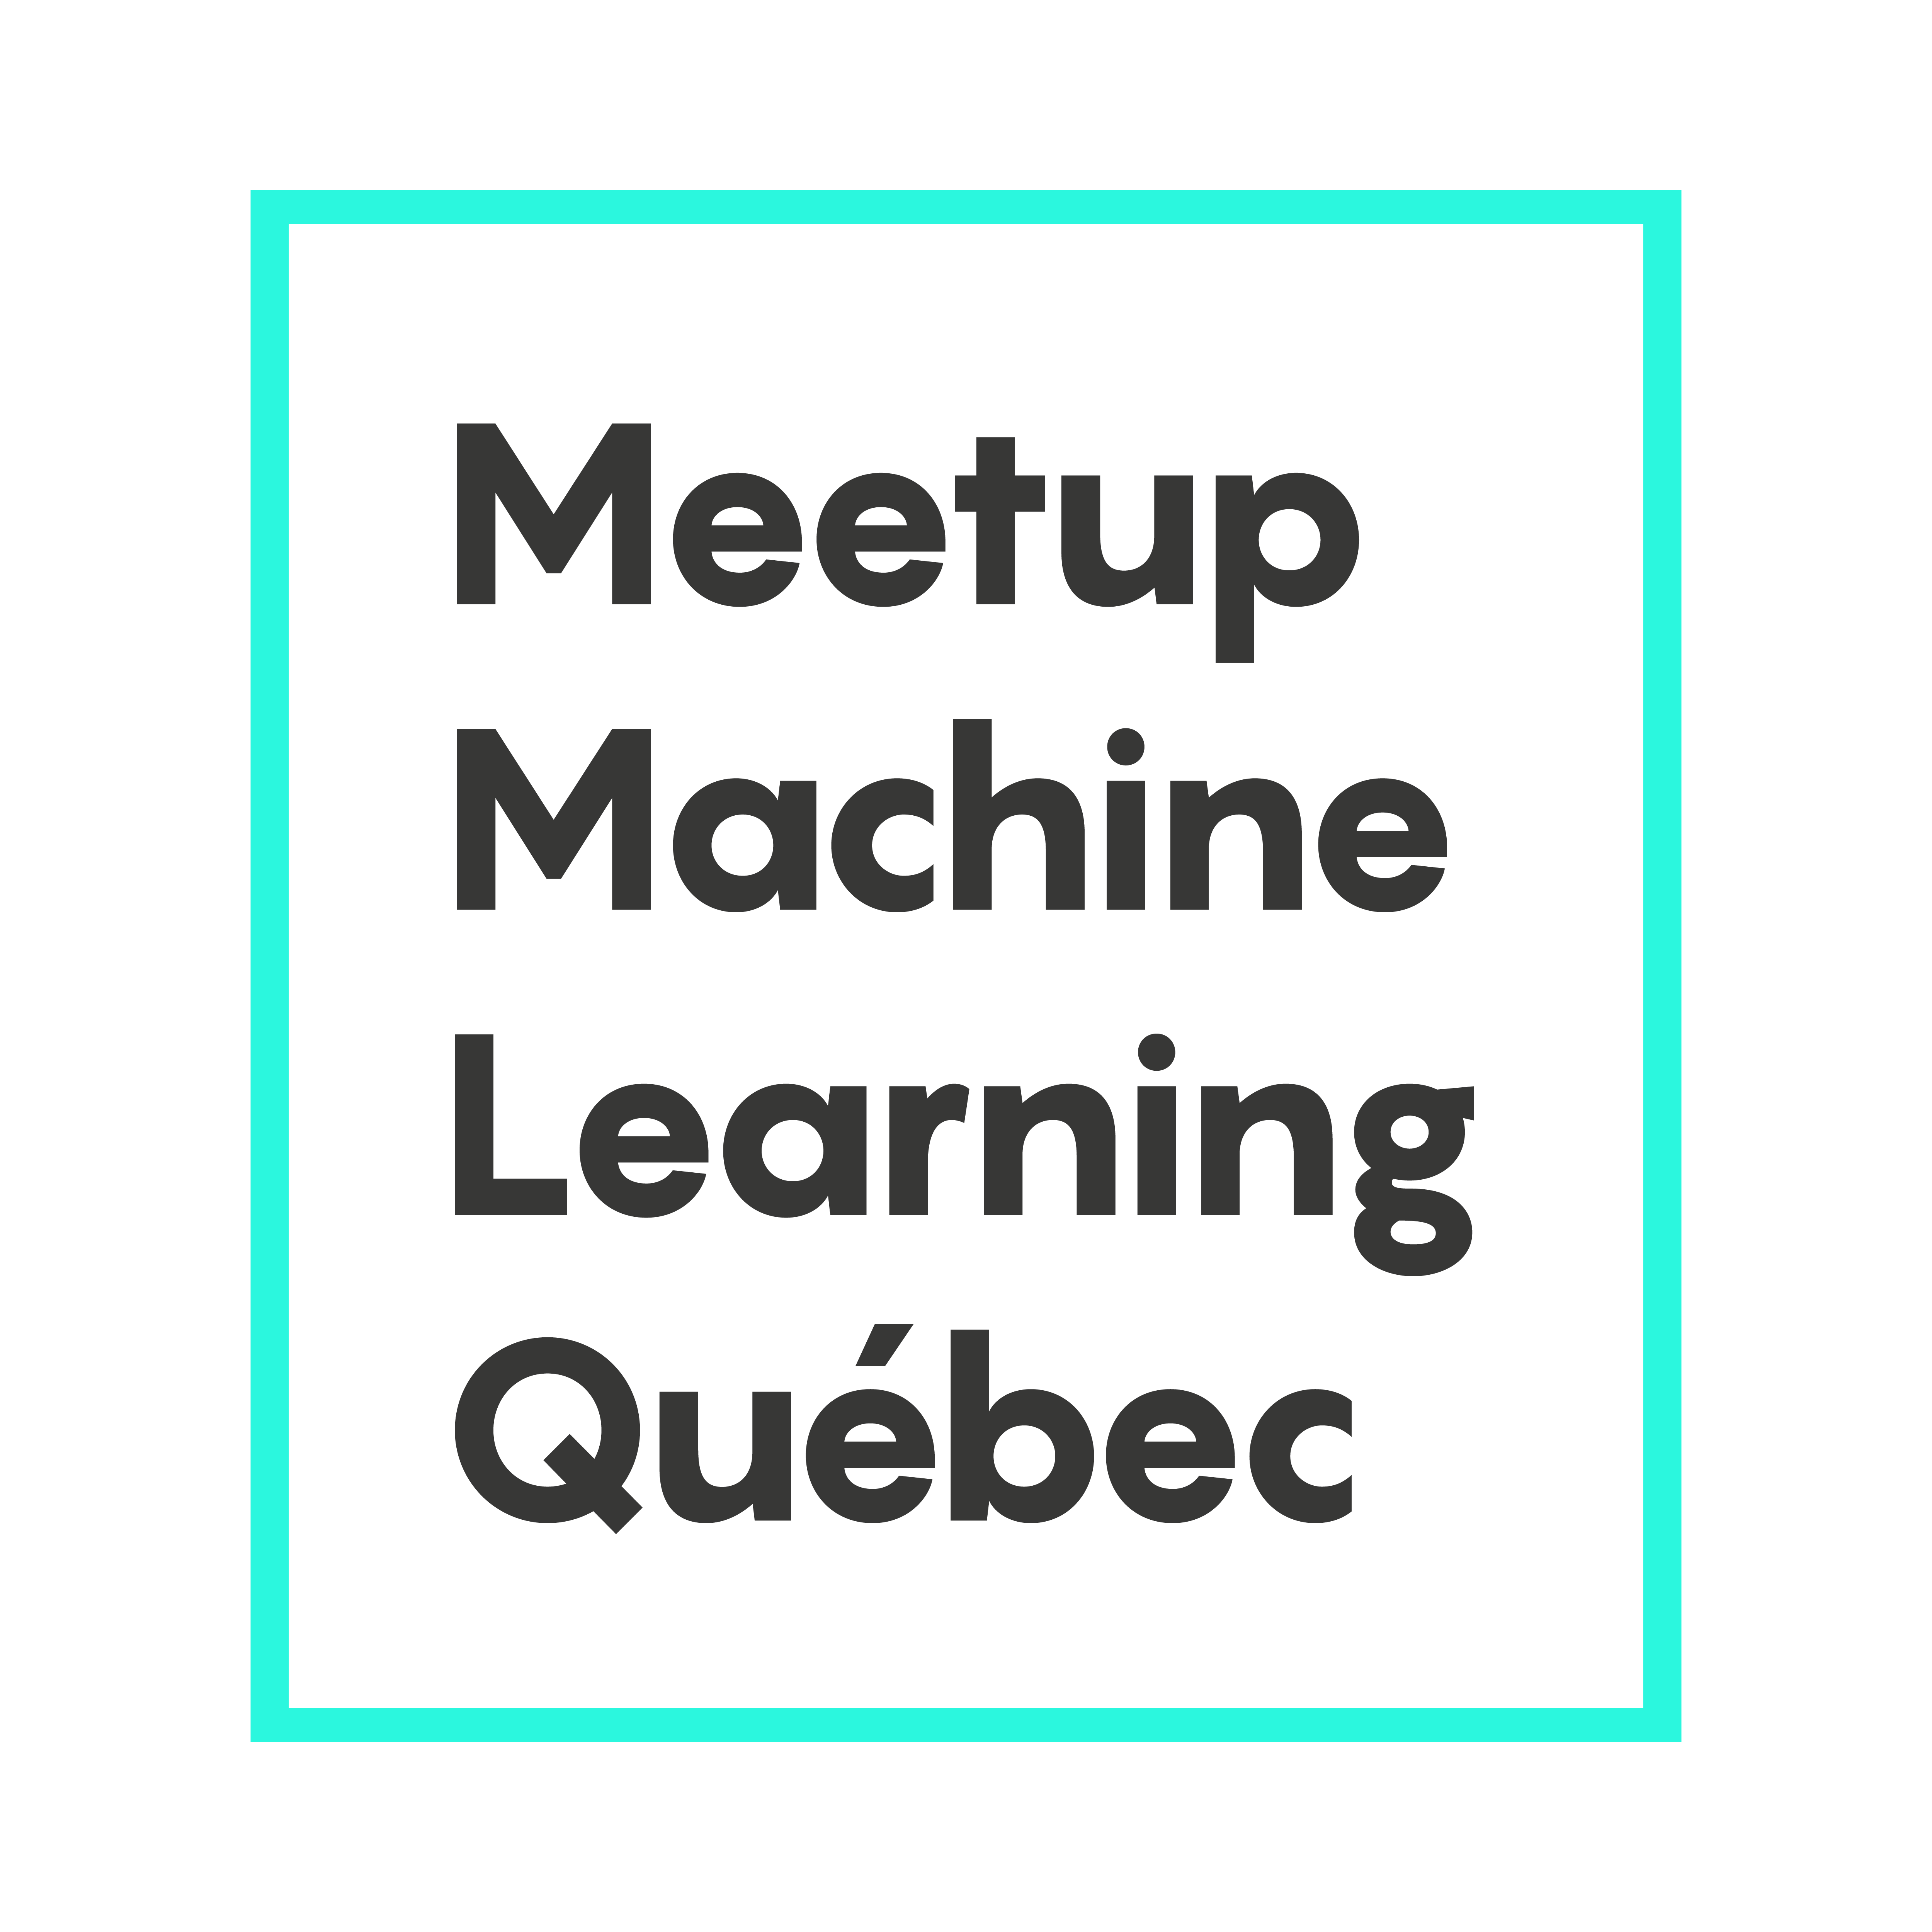
\includegraphics[scale=0.025]{images/meetup.png} \tab[0.8cm]}& Meetup Machine Learning Québec\\
	& Co-organisation des différents événements à Québec \\ 
	&\\[-6pt]

2019 -- 2020  &{\bf {Scientifique IA}}\\
\multirow{1}{*}{
\includegraphics[scale=0.09]{images/Vooban.png} \tab[1.15cm]}& Vooban\\
& Conseiller technique en intelligence artificielle \\ 
&\\[-6pt]
\end{tabular}

\subsection{Enseignement}
\begin{tabular}{L!{\VRule}R}
	2016 -- \tab[.7cm] &{\bf {Auxiliaire de cours}}\\
	\multirow{1}{*}{
\includegraphics[scale=0.1]{images/UL_P.pdf} \tab[0.6cm]}  &  Université Laval, École d'actuariat \\
	& Introduction à l'actuariat I, Gestion du risque financier I, Analyse et traitement collectif du risque, Informatique pour actuaire, Méthodes numériques en actuariat, Mathématiques actuarielles IARD II, Modèles linéaires en actuariat, Programmation avec R pour l'analyse de données \\ 
	&\\[-6pt]
	2019 -- 2020&{\bf {Auxiliaire d'enseignement}}\\
	\multirow{1}{*}{
\includegraphics[scale=0.1]{images/UL_P.pdf} \tab[0.6cm]}  &  Université Laval, CRDM - Centre de Recherche en Données Massives \\
	& École d'hiver en apprentissage automatique \\ 
	&\\[-6pt]
\end{tabular}

\subsection{Recherche}
\begin{tabular}{L!{\VRule}R}
2019 &{\bf {Auxiliaire de recherche}}\\
\multirow{1}{*}{
\includegraphics[scale=0.1]{images/UL_P.pdf} \tab[0.6cm]}  &  Université Laval, GRAAL \\
& Fusion d'enregistrements de risques commerciaux \\ 
& Luc Lamontagne, Chaire de recherche industrielle CRSNG - Intact Corporation financière sur l'apprentissage automatique en assurance\\ 
&\\[-6pt]
2019 &{\bf {Auxiliaire de recherche}}\\
\multirow{1}{*}{
\includegraphics[scale=0.1]{images/UL_P.pdf} \tab[0.6cm]}  &  Université Laval, GRAAL \\
& Apprentissage de taxonomie de compétences professionnelles \\ 
& Luc Lamontagne, Projet ENGAGE\\ 
&\\[-6pt]
2018 &{\bf {Auxiliaire de recherche}}\\
\multirow{1}{*}{
\includegraphics[scale=0.1]{images/UL_P.pdf} \tab[0.6cm]}  &  Université Laval, École d'actuariat \\
& Mesures reliées à l'indexation conditionnelle dans un régime de retraite à prestations déterminées \\ 
& Louis Adam, Chaire d'actuaire de l'Université Laval\\ 
&\\[-6pt]
2018 &{\bf {Auxiliaire de recherche}}\\
\multirow{1}{*}{
\includegraphics[scale=0.1]{images/UL_P.pdf} \tab[0.6cm]}  &  Université Laval, GRAAL \\
& Weighted bootstrapping method for word relation extraction  \\ 
& Luc Lamontagne\\ 
&\\[-6pt]
\end{tabular}

\section*{Publications}
\subsection*{\hspace{.5cm} Article}
\begin{tabular}{L!{\VRule}R}
2019 &  Nicolas Garneau, Mathieu Godbout, David Beauchemin, Audrey Durand, Luc Lamontagne. \href{https://arxiv.org/abs/1912.01706}{A Robust Self-Learning Method for Fully Unsupervised Cross-Lingual Mappings of Word Embeddings: Making the Method Robustly Reproducible as Well}. \textit{REPORLANG@LREC2020}.\\
&\\[-6pt]               
\end{tabular}

\vspace{4pt}

\subsection*{\hspace{.5cm} Non scientifique}

\begin{tabular}{L!{\VRule}R}
	2017 & David Beauchemin et Vincent Goulet \textit{\href{https://www.tug.org/TUGboat/Contents/contents38-3.html}{Typesetting actuarial symbols easily and consistently with actuarialsymbol and actuarialangle}}\\
	&\\[-6pt]  
\end{tabular}

\subsection*{\hspace{.5cm} Paquetages}

\begin{tabular}{L!{\VRule}R}
2019 & David Beauchemin \textit{\href{http://notificationdoc.ca/}{Notif: The notification package for every python project}}\\
&\\[-6pt] 
2017 & Simon-Pierre Gadoury et David Beauchemin \textit{\href{https://cran.r-project.org/web/packages/nCopula/index.html}{nCopula: Hierarchical Archimedean Copulas Through Multivariate Compound Distributions}} \\
&\\[-6pt]  
2017 & Vincent Goulet et David Beauchemin \textit{\href{http://ctan.org/pkg/actuarialsymbol}{actuarialsymbol - Actuarial notation with \LaTeX}}\\
&\\[-6pt] 
\end{tabular}

\vspace{10pt}


\section*{Communications}
\subsection*{\hspace{.5cm} Ateliers pratique}

\begin{tabular}{L!{\VRule}R}

2019 & \textbf{\href{http://raquebec.ulaval.ca/2019/event/les-tests-automatises-en-r}{Les tests automatisés en R}}\\
         & R à Québec\\
         &\\[-6pt]
2019 & \textbf{Extraction d'information à partir du Web}\\
	& Actulab\\
	&\\[-6pt]
2019 & \textbf{Atelier pratique en \faGit}\\
& Meetup Machine Learning Québec\\
&\\[-6pt]
2017 & \textbf{\href{https://vigou3.github.io/raquebec-atelier-introduction-r/}{Formation d'introduction à R}}\\
& R à Québec\\
&\\[-6pt]
2017 & \textbf{\href{https://davebulaval.github.io/R_Markdown/}{R \& Markdown}}\\
& École d'actuariat \\
&\\[-6pt]
\end{tabular}

\newpage

\subsection*{\hspace{.5cm} Conférences}

\begin{tabular}{L!{\VRule}R}
2020  & \textbf{Détection de doublon parmis des informations non structurées provenant de sources de données externes}\\
          &  Atelier scientifique Intact\\
          &  Université Laval, Canada \\
          &\\[-6pt]
2019 & \textbf{\href{https://davebulaval.github.io/bonnes-pratiques-git-material/}{Bonnes pratiques \& \faGit}}\\
	& IFT-6010 \\
	& Université Laval, Canada\\
	&\\[-6pt]
          
2019 & \textbf{\href{http://raquebec.ulaval.ca/2019/event/lassurance-qualite-et-le-calcul-scientifique}{Assurance Qualité, calcul scientifique \& R}}\\
	& R à québec \\
	& Université Laval, Canada\\
	&\\[-6pt]
2019 & \textbf{\href{http://raquebec.ulaval.ca/2019/event/lassurance-qualite-et-le-calcul-scientifique}{Assurance Qualité, calcul scientifique \& R}}\\
	& \href{https://www.ulaval.ca/les-etudes/chaires-de-leadership-en-enseignement-cle/les-chaires-de-leadership-en-enseignement/sciences-et-developpement-durable.html}{CLESSN} \\
	& Université Laval, Canada\\
	&\\[-6pt]
2019  & \textbf{Information gathering using external unstructured data sources}\\
	&  Atelier scientifique Intact\\
	&  Université Laval, Canada \\
	&\\[-6pt]
2019  & \textbf{Classification de doublons de risques commerciaux}\\
	&  Atelier scientifique Intact\\
	&  Université Laval, Canada \\
	&\\[-6pt]
2019 & \textbf{Introduction à Scikit-learn}\\
	& GRAAL summer school \\
	& Université Laval, Canada\\
	&\\[-6pt]
2018  & \textbf{Système de gestion des bénévoles Agapè}\\
	&  GLO-7035\\
	&  Université Laval, Canada \\
	&\\[-6pt]
2017  & \textbf{\href{https://github.com/davebulaval/Actulab_COOP}{Où sont les clients que nous ciblons?}}\\
	&  \href{http://www.actulab.ca}{Actulab}\\
	&  Université Laval, Canada \\
	&\\[-6pt]
\end{tabular}

\vspace{10pt}

\section*{Bourses}
\begin{tabular}{L!{\VRule}R}
2020 & \textbf{Bourse de recherche} \\
		& Chaire de recherche industrielle CRSNG-Intact Corporation financière sur l'apprentissage machine en assurance\\
        & Développement logiciel de la librairie Poutyne \\
        &\\[-6pt]
2019 & \textbf{Bourse de recherche} \\
	& Chaire de recherche industrielle CRSNG-Intact Corporation financière sur l'apprentissage machine en assurance\\
	& Développement logiciel de la librairie Poutyne\\
	&\\[-6pt]
2019 & \textbf{Bourse de recherche} \\
	& Chaire de recherche industrielle CRSNG-Intact Corporation financière sur l'apprentissage machine en assurance\\
	& Fusion d'enregistrements de risques commerciaux\\
	&\\[-6pt]  
2018 & \textbf{Bourse d'excellence Gaston Paradis} \\
	& Université Laval\\
	& Implication sociale\\
	&\\[-6pt]
2018 & \textbf{Bourse Yves-Roy} \\
	& Université Laval\\
	& Meilleure projet en génie logiciel orienté-objet\\
	&\\[-6pt]       
\end{tabular}

\newpage
\section*{Prix et distinction}
  
\begin{tabular}{L!{\VRule}R}
2016 -- 2018 & \textbf{Gala du mérite étudiant} \\
	& AESGUL\\
	& Implication sociale\\
	&\\[-6pt]         
\end{tabular}

 \vspace{10pt}

\section*{Implications}
\subsection*{\hspace{.5cm} Comité}
\begin{tabular}{L!{\VRule}R}
2020 -- \tab[.7cm] & \textbf{Comité d'organisation de R à Québec}\\
	& Président du comité d'organisation des ateliers pratiques \\
	& Université Laval, Canada\\
	&\\[-6pt]
2020 -- \tab[.7cm] & \textbf{Comité éditorial}\\
	& Président du comité d'éditorial du blogue \\
	& \href{https://www.dotlayer.org/}{.Layer}\\
	&\\[-6pt]
2020 -- \tab[.7cm] & \textbf{Comité Data Universal Tool}\\
	& Président du comité de développement de Data Universal Tool \\
	& \href{https://www.dotlayer.org/}{.Layer}\\
	&\\[-6pt]
2020 & \textbf{Atelier de co-design prospectif}\\
	& Participation \\
	& OBVIA - Observatoire international sur les impacts sociétaux de l'IA et du numérique\\
	&\\[-6pt]
2019 -- 2020 & \textbf{Comité d'amélioration des évaluations d'enseignement}\\
	& Faculté des sciences et du génie, Université Laval\\
	&\\[-6pt]
2018 & \textbf{Comité d'organisation de la semaine de l'apprentissage automatique en assurance}\\
	& Meetup Machine Learning Québec\\
	&\\[-6pt]
\end{tabular}

\vspace{4pt}

\subsection*{\hspace{.5cm} Jury}
\begin{tabular}{L!{\VRule}R}
2018 -- \tab[.7cm] & \textbf{Membre du jury}\\
	& Mon Travail pratique en 180 secondes \\
	& École d'actuariat, Université Laval\\
	&\\[-6pt]
2019 -- \tab[.7cm] & \textbf{Membre du jury}\\
& Présentation des projets de session\\
& Département d'informatique, Université Laval\\
&\\[-6pt]
\end{tabular}

\vspace{4pt}

\subsection*{\hspace{.5cm} Coopérative}
\begin{tabular}{L!{\VRule}R}
2020 -- \tab[.7cm]  & \textbf{\href{https://baseline.quebec/}{Baseline}} \\
	\multirow{1}{*}{
\includegraphics[scale=0.075]{images/Baseline.png} \tab[1.1cm]} & Président du conseil d'administration de la coopérative de travailleurs Baseline en intelligence artificielle\\
	& Québec, Canada\\
	&\\[-6pt]
\end{tabular}
\vspace{4pt}
\subsection*{\hspace{.5cm} Organisme à but non lucratif}
\begin{tabular}{L!{\VRule}R}
2019 -- \tab[.7cm]  & \textbf{\href{https://www.dotlayer.org/}{.Layer}} \\
	\multirow{1}{*}{
\includegraphics[scale=0.055]{images/DotLayer.png} \tab[1cm]}& Vice-président aux développements des affaires\\
	& Québec, Canada\\
	&\\
	&\\[-6pt]                      
2016 -- 2018 & \textbf{AÉACT - Association des étudiants en actuariat de l'Université Laval}\\
	& Université Laval, Canada\\
	&\\[-6pt]
\end{tabular}

\vspace{4pt}

\subsection*{\hspace{.5cm} Balado}
\begin{tabular}{L!{\VRule}R}
	2020 -- \tab[.7cm] & \textbf{IA \& café}\\
	&Animateur invité au podcast IA \& café
\end{tabular} \\
\end{document}